\begin{apendicesenv}

\partapendices

\chapter{Grafos}

\section{Um Pouco mais de História}

Graças à resolução dada por Euler, mais tarde muitos outros problemas importantes, para o desenvolvimento da Matemática Aplicada, foram possíveis de serem modelados. Um desses modelos são as relações de amizade, de hierarquia, de trabalho. Netto \cite{Netto:2012}, aponta grafos como um auxílio para o estudo de problemas envolvendo inter-relacionamento de elementos (em química orgânica, eletricidade, organização, transporte, psicossociologia). Na verdade, grafos modelam diversas situações e muitas delas não quantificáveis.

Conforme Ore \cite{Ore:1963}, o matemático irlandês William Hamilton, em 1859, inventou um jogo chamado ``\textit{The Icosian Game}'', com um peculiar enigma envolvendo um dodecaedro, em que cada um dos 20 vértices foram nomeados com nomes de cidades importantes. O objetivo do jogo era, utilizando as 30 arestas do dodecaedro, passar por cada uma das cidades apenas uma vez, começando e terminando na mesma cidade. Um exemplo do grafo pode ser visualizado na figura \ref{grafo_hamiltoniano}.

\begin{figure}[!h]
	\centering
	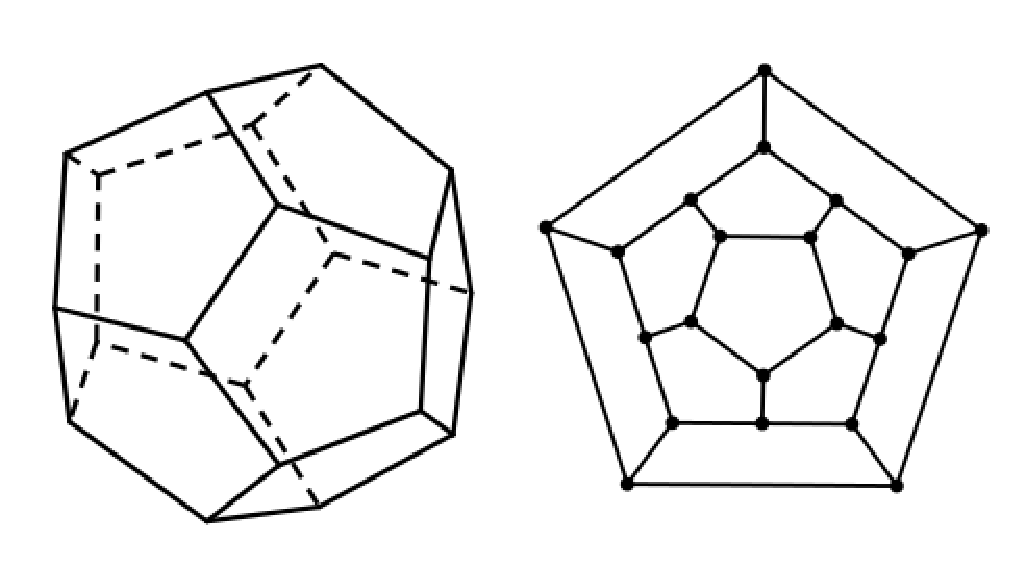
\includegraphics[scale=0.3]{figuras/capitulo2/grafo_hamiltoniano.eps}
	\caption[Grafo hamiltoniano]{Grafo hamiltoniano \cite{Ore:1963}}
	\label{grafo_hamiltoniano}
\end{figure}

Apesar da simples formulação, o problema admite muitos caminhos como resposta. No problema de Hamilton, temos uma diferença significativa em relação ao problema de Euler. Encontrar um caminho euleriano significa encontrar um caminho que passe por todas as arestas do grafo uma única vez, podendo ser aberto ou fechado. Nos caminhos hamiltonianos, cada vértice é visitado uma única vez. O problema fica mais complexo com tal condição \cite{Costa:2011}.

\section{Outras Definições}

Um grafo é finito se tanto o seu conjunto de vértices, quanto o seu conjunto de arestas são finitos. Um grafo sem vértices (e, portanto, sem arestas) é o grafo nulo. Qualquer grafo apenas com um vértice é referido como trivial. Todos os outros grafos são não-triviais \cite{Costa:2011}.

Um grafo é simples se não tem \textit{loops} ou arestas paralelas \cite{Diestel:1997}, como exemplificado na figura \ref{grafo_simples}.

\begin{figure}[!h]
	\centering
	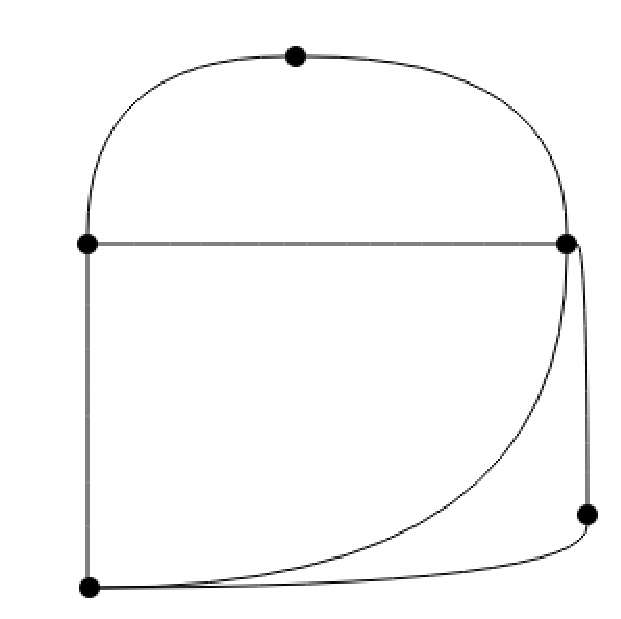
\includegraphics[scale=0.2]{figuras/capitulo2/grafo_simples.eps}
	\caption[Exemplo de grafo simples]{Exemplo de grafo simples \cite{Costa:2011}}
	\label{grafo_simples}
\end{figure}

Certos tipos de grafos podem desempenhar papéis proeminentes na teoria dos grafos. Um grafo conexo é um grafo simples no qual quaisquer dois vértices são ligados por um caminho. Um grafo é vazio quando não há dois vértices adjacentes (isto é, o conjunto de arestas é vazio). Um grafo é bipartido se o seu conjunto de vértices pode ser particionado em dois subconjuntos \textit{X} e \textit{Y} para que cada aresta tem um fim em \textit{X} e um fim em \textit{Y}; uma tal partição (\textit{X}, \textit{Y}) é chamada uma bipartição do grafo, e \textit{X} e \textit{Y} suas partes. Pode-se denotar um grafo bipartido \textit{G} com bipartição (\textit{X}, \textit{Y}) por \textit{G}[\textit{X}, \textit{Y}]. Se \textit{G}[\textit{X}, \textit{Y}] é simples e todos os vértices de \textit{X} estão associados a cada vértice em \textit{Y}, então \textit{G} é chamado de um grafo bipartido completo. Uma estrela é um grafo bipartido completo \textit{G}[\textit{X}, \textit{Y}] com |\textit{X}| = 1 ou |\textit{Y}| = 1 \cite{Diestel:1997}.  A figura \ref{tipos_grafos} ilustra estes tipos de grafos, sendo o grafo ``A'' é um grafo conexo, o grafo ``B'' é um grafo vazio e o grafo ``C'' é um grafo bipartido completo.

\begin{figure}[!h]
	\centering
	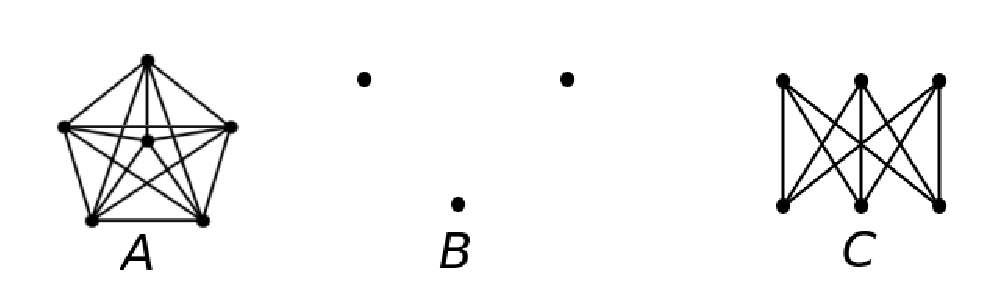
\includegraphics[scale=0.4]{figuras/capitulo2/tipos_grafos.eps}
	\caption[Tipos de grafos]{Tipos de grafos \cite{Diestel:1997}}
	\label{tipos_grafos}
\end{figure}

Um caminho é um grafo simples cujos vértices podem ser dispostos em uma sequência linear. De tal forma que dois vértices são adjacentes se forem consecutivos na sequência, e não adjacentes caso não forem consecutivos \cite{Bondy:2007}. Dessa forma, diz-se que um vértice é alcançável a partir de outro, se houver um caminho levando o primeiro vértice ao último \cite{Costa:2011}. A figura \ref{caminho} apresenta um caminho (arestas em vermelho) do vértice ``a'' até o vértice ``e''.

\begin{figure}[!h]
	\centering
	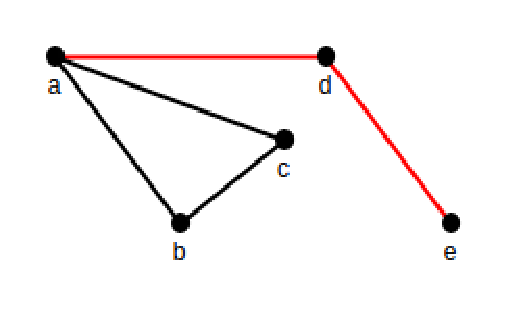
\includegraphics[scale=0.5]{figuras/capitulo2/caminho.eps}
	\caption[Caminho]{Caminho \cite{Costa:2011}}
	\label{caminho}
\end{figure}

Do mesmo modo, um ciclo é um grafo simples cujos vértices podem ser dispostos em uma sequência cíclica de tal maneira que dois vértices são adjacentes se forem consecutivos na sequência. O comprimento de um caminho ou de um ciclo é o número de suas arestas \cite{Costa:2011}. É possível observar na figura \ref{ciclos} alguns exemplos de grafos com ciclo.

\begin{figure}[!h]
	\centering
	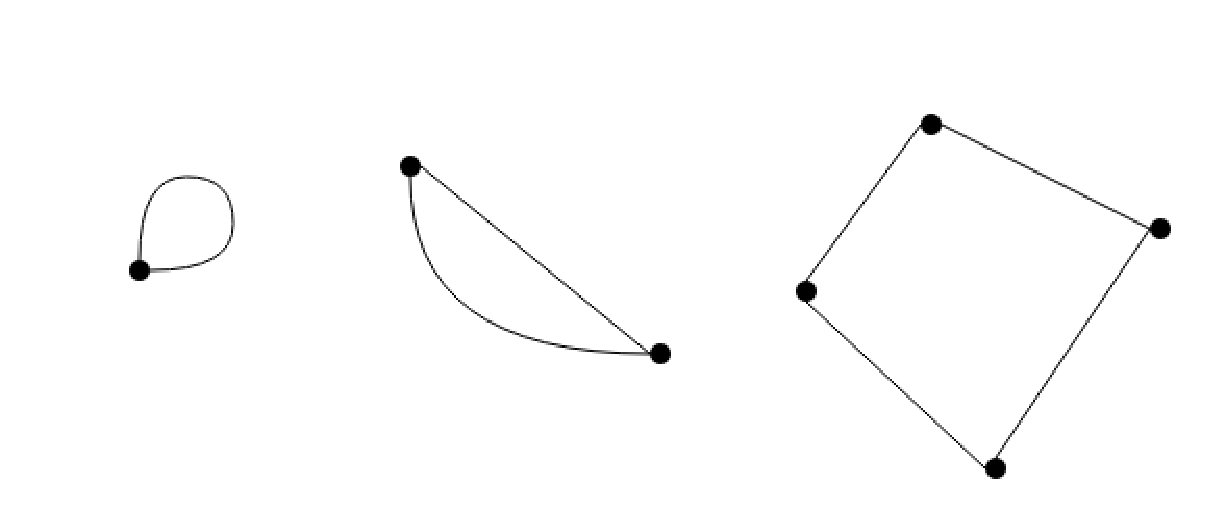
\includegraphics[scale=0.3]{figuras/capitulo2/ciclos.eps}
	\caption[Exemplo de grafos com ciclos]{Exemplo de grafos com ciclos \cite{Costa:2011}}
	\label{ciclos}
\end{figure}

Um grafo é conectado se, para cada partição de seus vértices definido em dois conjuntos \textit{X} e \textit{Y} não vazios, existe uma aresta com uma extremidade em \textit{X} e uma extremidade em \textit{Y}; caso contrário, o grafo é desconectado. Em outras palavras, um grafo é desconectado se o conjunto de vértices pode ser particionado em dois subconjuntos não vazios \textit{X} e \textit{Y} e que nenhuma aresta tem uma extremidade em \textit{X} e a outra extremidade em \textit{Y}. É instrutivo comparar esta definição com a de um grafo bipartido. Os exemplos de grafos conectados e desconectados são apresentados na figura \ref{desconectados}, onde o grafo ``X'' e o grafo ``Y'' são dois grafos distintos conectados. Porém se fossem trados como um único grafo, este seria um grafo desconectado \cite{Bondy:2007}.

\begin{figure}[!h]
	\centering
	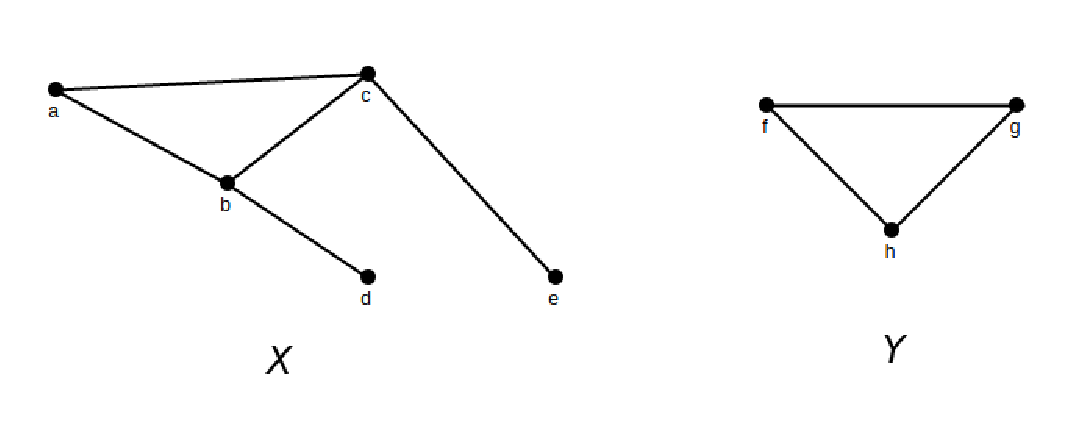
\includegraphics[scale=0.45]{figuras/capitulo2/desconectados.eps}
	\caption[Exemplo de grafos conectados e desconectados]{Exemplo de grafos conectados e desconectados \cite{Bondy:2007}}
	\label{desconectados}
\end{figure}

O grau de um vértice \textit{v} em um grafo \textit{G}, designado por \textit{d$_G$}(\textit{v}), é o número de arestas de \textit{G} que incidem em \textit{v}; para cada \textit{loop} é contado duas arestas. Em particular, se \textit{G} é um grafo simples, \textit{d$_G$}(\textit{v}) é o número de vizinhos de \textit{v} em \textit{G}. Um vértice de grau zero é chamado um vértice isolado. Denominamos por $\delta$(\textit{G}) e $\Delta$(\textit{G}) mínimo e máximo graus dos vértices de \textit{G}, e por \textit{d}(\textit{G}), o seu grau médio, $\frac{1}{n}\sum_{\textit{v}\in\textit{V}} \textit{d}(\textit{v})$ \cite{Diestel:1997}.

\chapter{Reutilização de Software}

\section{Padrão Abstract Factory}
\label{sec:padrao_abstract_factory}

A seguir, têm-se uma breve descrição do padrão ``\textit{Abstract Factory}'', como foi definido em \cite{Gamma:1995}.

Esse padrão fornece uma estrutura para criação de famílias de objetos relacionados sem a necessidade de definir suas classes concretas. A figura \ref{abstract_factory} apresenta o modelo do ``\textit{Abstract Factory}''.

\begin{figure}[!h]
	\centering
	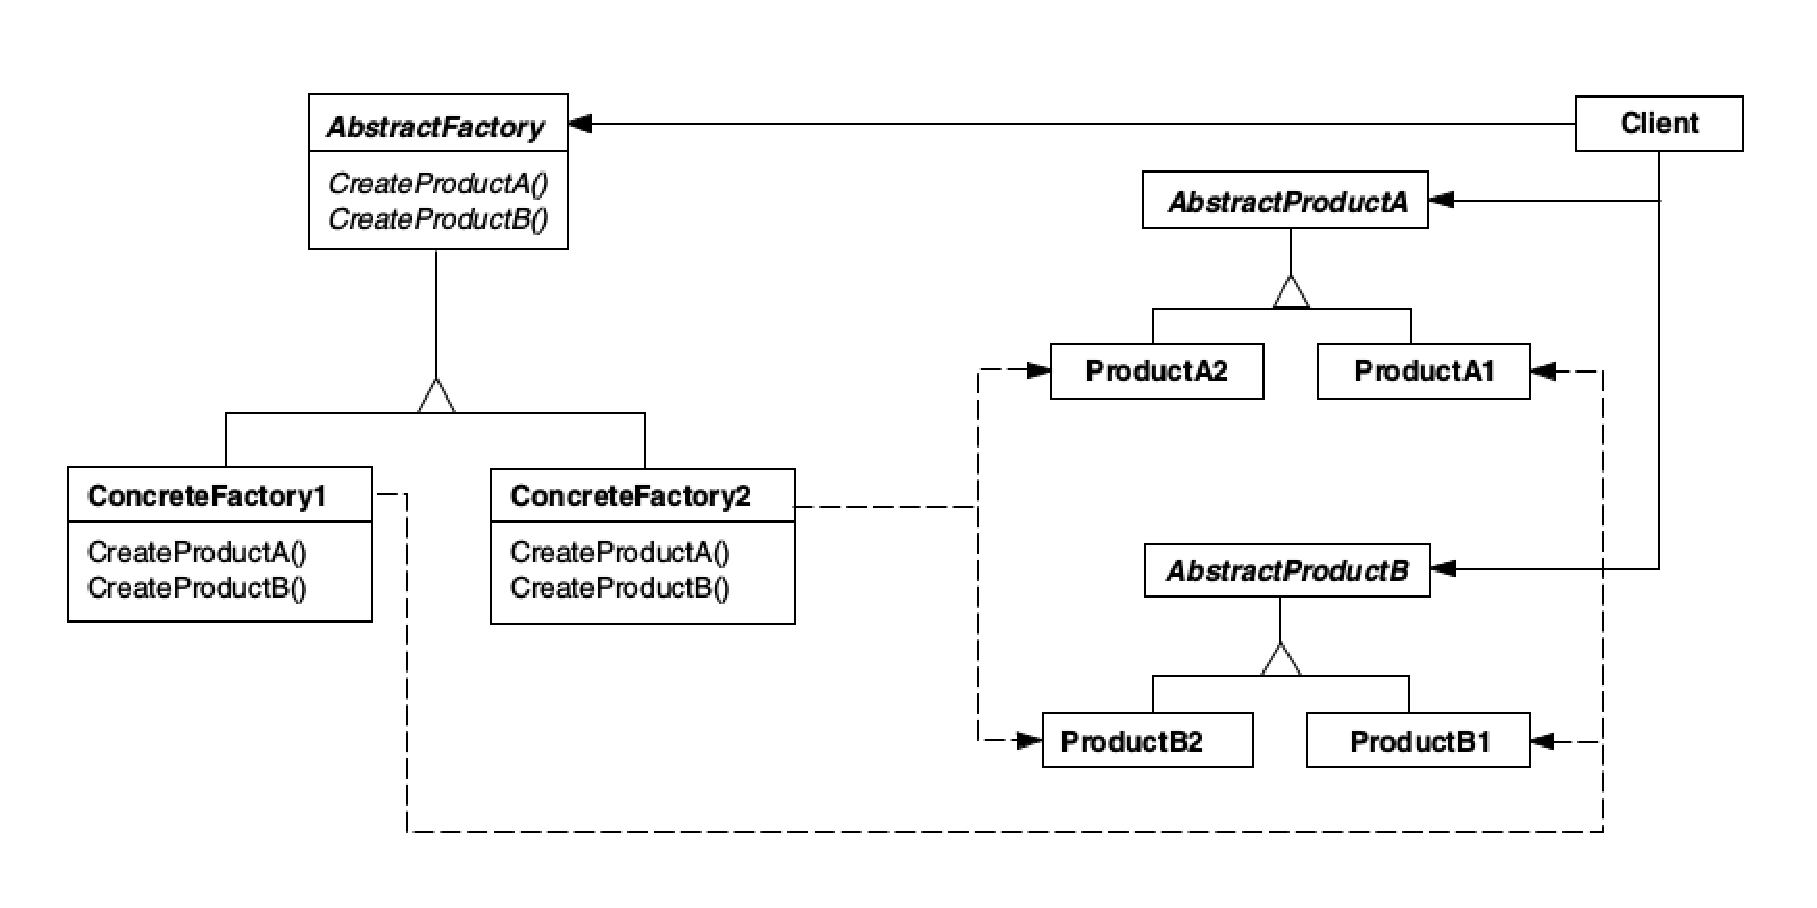
\includegraphics[scale=0.5]{figuras/apendices/abstract_factory.eps}
	\caption[Modelo genérico do Abstract Factory]{Modelo genérico do Abstract Factory \cite{Gamma:1995}}
	\label{abstract_factory}
\end{figure}

O modelo da figura apresenta cinco tipos de classes. ``\textit{Abstract Factory}'', ``\textit{Concrete Factory}'', ``\textit{Abstract Product}'', ``\textit{Product}'' e ``\textit{Client}''.

\begin{itemize}
	\item \textbf{\textit{Abstract Factory:}} Faz declarações de interfaces para criação de quaisquer produtos;
	\item \textbf{\textit{Concrete Factory:}} Essas classes já estão focadas no tipo de produtos que vão criar e implementam os métodos abstratos para essa criação;
	\item \textbf{\textit{Abstract Product:}} Classes abstratas que declaram interfaces para um determinado tipo de produto que deverá ser criado;
	\item \textbf{\textit{Product:}} Classes que representam o próprio produto que deverá ser criado, são as classes que são chamadas pelos métodos de criação presentes nas ``\textit{Concrete Factory}'';
	\item \textbf{\textit{Client:}} É a classe que representa quem irá fazer as chamadas aos métodos de criação. Não é necessário que conheça de fato as classes concretas de produto, pois apenas faz uso das interfaces declaradas em ``\textit{Abstract Factory}'' e ``\textit{Abstract Product}''; a primeira para criar os produtos, e a segunda para usá-los.
\end{itemize}

Este padrão oferece algumas vantagens e desvantagens que são apresentadas a seguir:

\begin{itemize}
	\item \textbf{Isolamento de classes concretas:} O cliente pode trabalhar com as criações dos produtos sem necessariamente conhecer as classes concretas que existem por traz, pois este trabalha apenas com as interfaces abstratas providas.
	\item \textbf{Fácil troca de famílias de produtos:} Basta trocar qual é a classe concreta que deverá ser usada que todo o comportamento dos produtos irá se alterar de acordo com essa classe. Isso pode ser feito facilmente no momento de instanciação da fábrica.
	\item \textbf{Harmonia entre produtos:} Como o padrão permite aos clientes trabalharem apenas com uma família por vez, fica fácil alcançar harmonia, pois todos os produtos da família estão de alguma forma relacionados.
	\item \textbf{Suporte a novos tipos de produtos é difícil:} Como a interface do ``\textit{Abstract Factory}'', no início, cria uma quantidade fixa de produtos para serem implementados, alterar isso fica difícil, pois é necessário mexer na classe principal e criar as subclasses concernentes.
\end{itemize}

\section{Padrão Factory Method}
\label{sec:padrao_factory_method}

Um outro padrão de criação bem parecido com o \nameref{sec:padrao_abstract_factory}, porém, diferentemente do anterior que cria famílias de objetos, o \textit{Factory Method} é responsável por criar um único objeto \cite{Gamma:1995}. A figura \ref{factory_method} apresenta o modelo de classes desse padrão:

\newpage
\begin{figure}[!h]
	\centering
	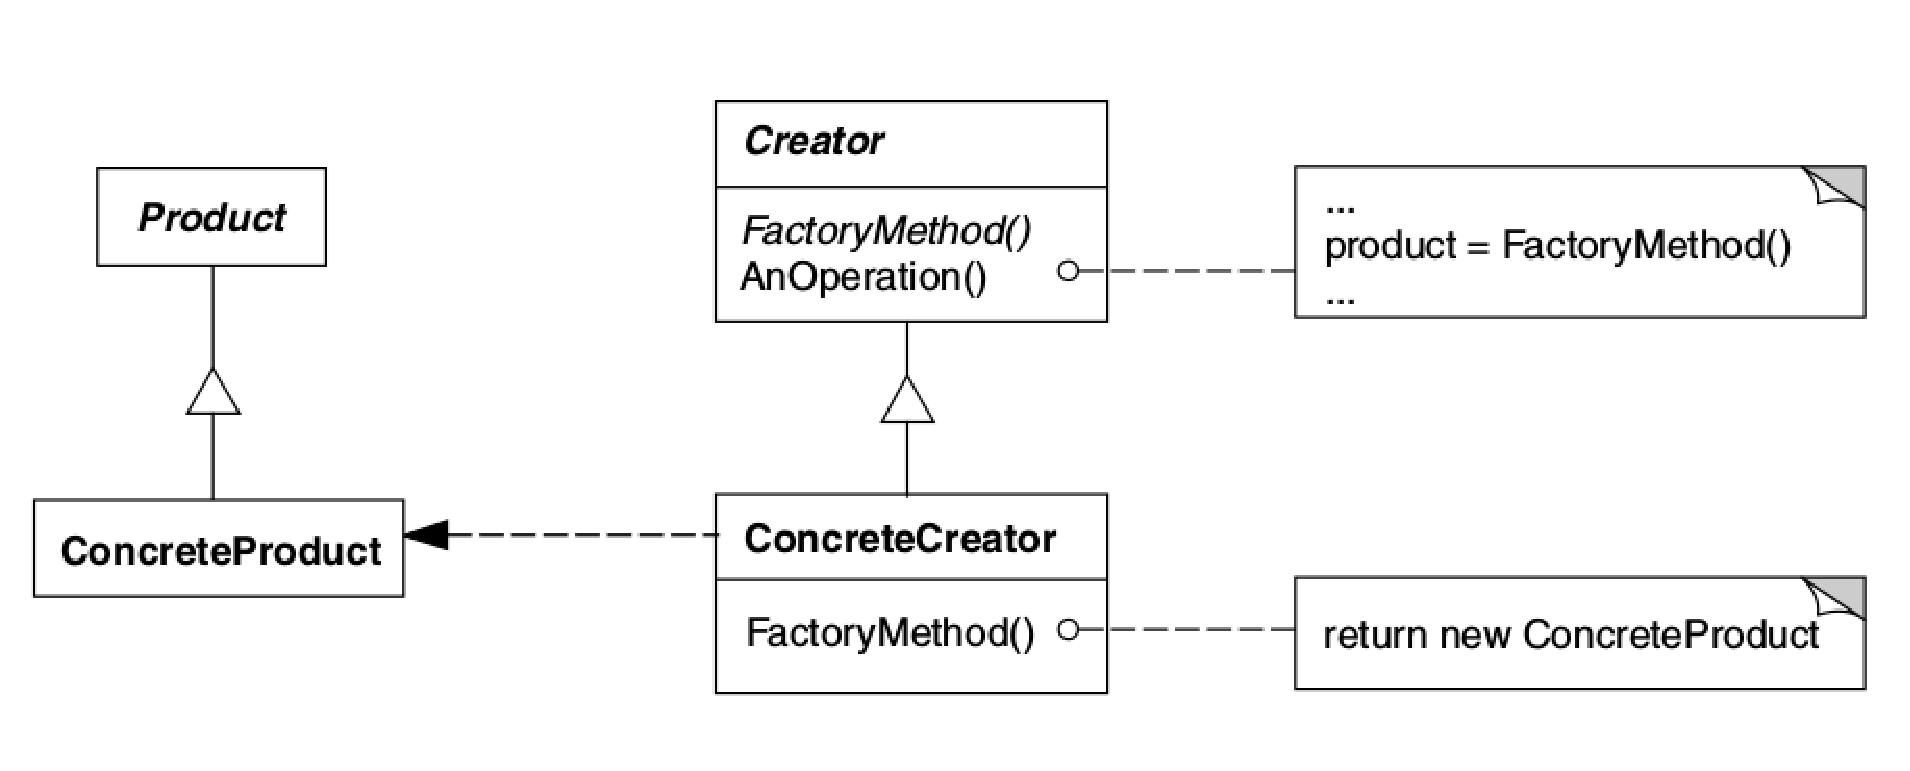
\includegraphics[scale=0.5]{figuras/apendices/factory_method.eps}
	\caption[Modelo genérico do Factory Method]{Modelo genérico do Factory Method \cite{Gamma:1995}}
	\label{factory_method}
\end{figure}

Com esse padrão fica fácil e prático fazer a alteração de uma sub-classe concreta, uma vez que, a aplicação passa a trabalhar com a interface de ``\textit{Product}'', o código pode trabalhar com quaisquer classes ``\textit{ConcrectProduct}'' definidas pelo usuário.

As classes mostradas no modelo são descritas a seguir:

\begin{itemize}
	\item \textbf{\textit{Product}}: Interface de objetos que o método de fábrica irá criar;
	\item \textbf{\textit{ConcretProduct}}: Implementação da interface ``\textit{Product}'';
	\item \textbf{\textit{Creator}}: Interface com método para criação de um ``\textit{Product}'';
	\item \textbf{\textit{ConcrectCreator}}: Implementação da interface ``\textit{Creator}'', reimplementa o método para criação de um ``\textit{ConcrectProduct}''.
\end{itemize}

\section{Padrão Strategy}
\label{sec:padrao_strategy}

O padrão ``\textit{Strategy}'' foi desenvolvido para auxiliar desenvolvedores a trabalhar com famílias de algoritmos que podem variar independentemente dos clientes que os usam \cite{Gamma:1995}. Com esse padrão é possível mudar facilmente o comportamento de um dado algoritmo apenas trocando a classe que é usada na implementação do mesmo. A seguir é apresentado o modelo de classes desse padrão na figura \ref{strategy}.

\newpage
\begin{figure}[!h]
	\centering
	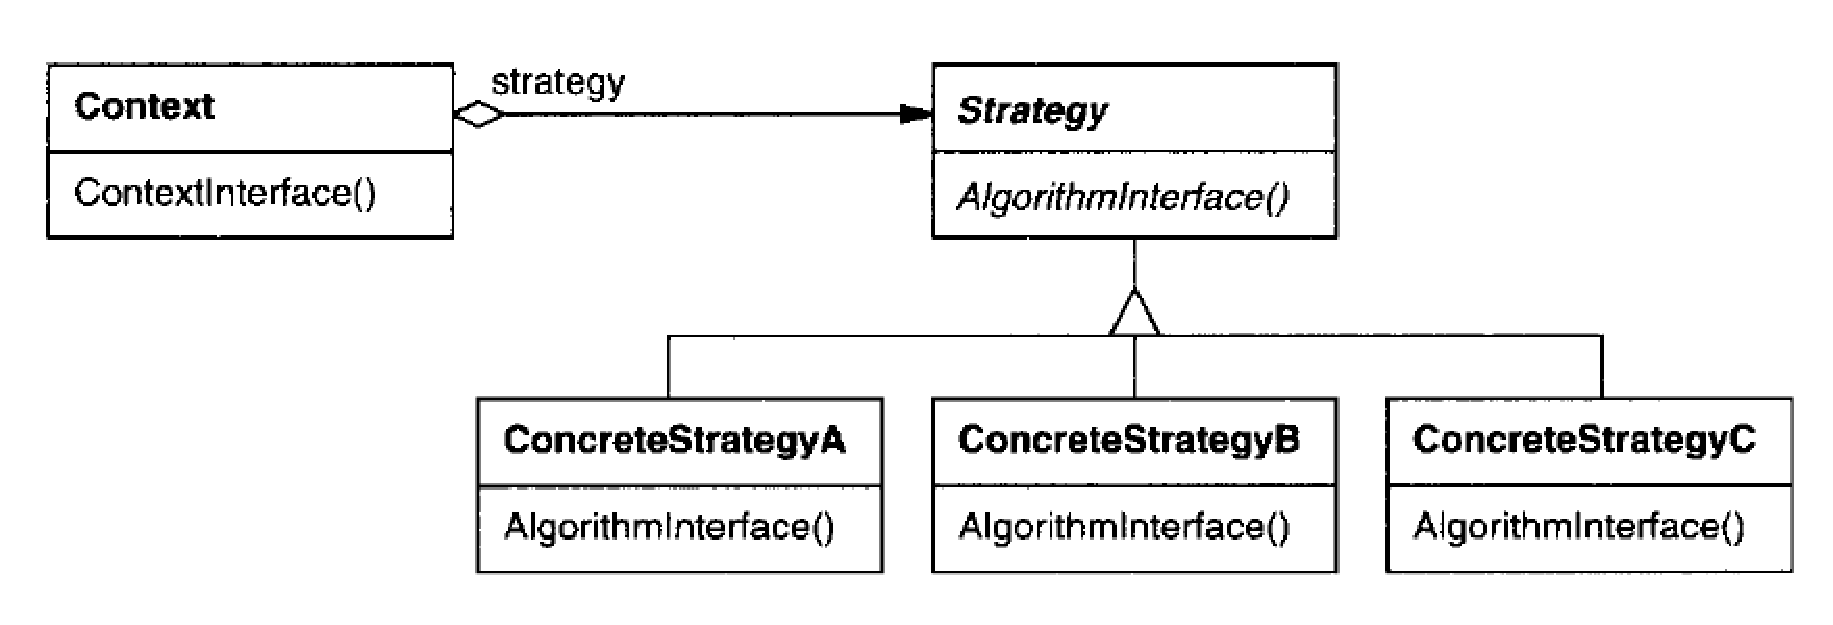
\includegraphics[scale=0.5]{figuras/apendices/strategy.eps}
	\caption[Modelo genérico do Strategy]{Modelo genérico do Strategy \cite{Gamma:1995}}
	\label{strategy}
\end{figure}

As classes do modelo são descritas a seguir.

\begin{itemize}
	\item \textbf{\textit{Strategy}}: Interface comum para todos os algoritmos que serão suportados.
	\item \textbf{\textit{ConcretStrategy}}: Implementação da interface ``\textit{Strategy}'' definindo cada método com um comportamento esperado para um determinado cliente;
	\item \textbf{\textit{Context}}: Essa classe faz uso da interface ``\textit{Strategy}'' chamando cada um de seus métodos através de um objeto ``\textit{ConcretStrategy}'' que é definido, sendo assim,  o comportamento esperado será retornado de acordo com o ``\textit{ConcretStrategy}'' que é passado.
\end{itemize}

\end{apendicesenv}
